\ifpdf
    \graphicspath{{Chapter_2006/figures/PNG/}{Chapter_2006/figures/PDF/}{Chapter_2006/figures/}}
\else
    \graphicspath{{Chapter_2006/figures/EPS/}{Chapter_2006/figures/}}
\fi

\newpage\section{Discussion}\label{sec:2006/discussion}

\subsection{Tracer relations}\label{ssec:2006/discuss/tracer}

	\begin{wrapfigure}{o}{0.5\textwidth}
		\centering
		\vspace{-.3in}
		\begin{singlespacing}
		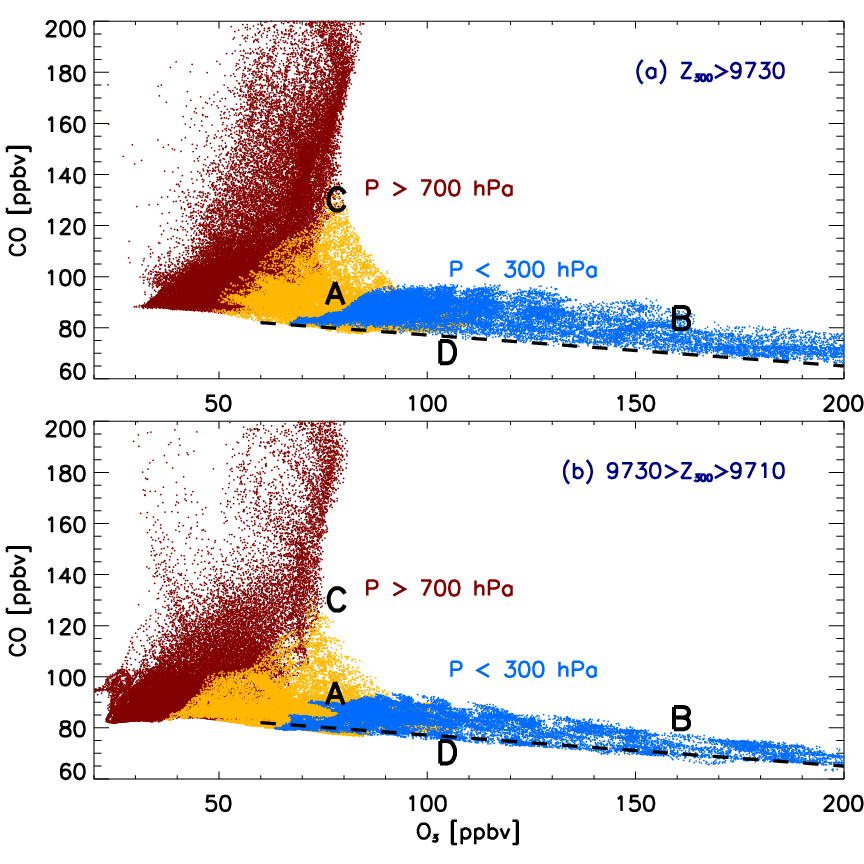
\includegraphics[width=0.48\textwidth]{tracer/tracer_correlations}
		\caption[\chem{CO}-\chem{O_3} model correlation]{{\label{fig:2006/o3co}\small\textbf{\chem{CO}-\chem{O_3}
		model correlation} --- \textbf{(a)} Anticyclone ($\bar{Z}_{300}>9730\,\unit{m}$) \chem{CO}-\chem{O_3}(adjusted)
		joint-distribution separately colored by pressure levels: red below 700\,\unit{hPa}, blue above 300\,\unit{hPa}, and yellow in between. \textbf{(b)} Same as \textbf{a} but outside the anticyclone
		between 9710\,\unit{m} and 9730\,\unit{m}. Data points south of 25$^\circ$N have been removed to reduce impact
		of the southern boundary. \vspace{-.3in}}}
		\end{singlespacing}
	\end{wrapfigure}

The relationship between ozone and carbon monoxide (\chem{CO}) has been used to study tropospheric-stratospheric transition in
chemical regimes \citep[e.g.][and references therein]{Pan:2007sw,Hegglin:2009fk}. Similarly, such analysis may be applied to tropospheric data
alone to identify contributions from various pathways \citep[e.g.][]{Zhang:2006zr,Voulgarakis:2011fk,Cristofanelli:2013uq}. Ignoring
\chem{NO_x}, ozone is expected to be strongly positively correlated with \chem{CO} \citep[][, see also Ch.~\ref{ch:introduction}]{Chin:1994kx}. However, since the dominating
source for \chem{CO} is surface emission, boundary layer dynamics strongly limit \chem{CO}'s concentration in the upper troposphere.
On the other hand, near the tropopause, contribution of stratospheric ozone and upper tropospheric production cause ozone to
increase rapidly with height. Together, \chem{O_3-CO} anti-correlation over a sufficiently expansive column can expect to observe
an "L"-shaped joint distribution.

Here we examine the joint-distribution of the August average model ozone and \chem{CO} from the surface up to 100\,\unit{hPa} (Fig.~\ref{fig:2006/o3co}).
Data points are first separated by within and outside of the anticyclone, defined by the boundary $\bar{Z}_{300}$ as previously
defined in Section~\ref{ssec:2006/gen/ozone}. Then, each panel is further classified by pressure levels split at 300 and 700\,\unit{hPa}
to represent the lower, middle, and upper troposphere. To account for model biases, ozone VMRs between 100--300\,\unit{hPa}
have been adjusted by the differences in mean and variance against TES computed in Section~\ref{ssec:2006/gen/ozone}. No
adjustment is performed at the other pressure levels due to insignificant bias compared to observations.
The shape and features of the joint-distribution remain consistent before and after the adjustment. The labeled features annotated
in the figure are discussed below.

Feature A indicates a type of air mass exist only outside the anticyclone. By identifying the locations and timing of these data points,
this feature is identified to be corresponding to subtropical Atlantic
influx from the southern boundary. Typically, it has higher \chem{CO} but the ozone VMRs at 300\,\unit{hPa} from lower latitudes are
lower in general. These air masses intermittently contribute to the anticyclone, similar to the air masses mixed across the jet stream
from the north (see Sect.~\ref{ssec:2006/gen/ozone} \& \ref{ssec:2006/gen/co}). Feature B indicates the upper tropospheric branch
of the \chem{O_3}-\chem{CO} distribution. It is evident from the labels, which are placed at the same locations in both panels, that
\chem{CO} is more effective in raising the ozone level within the upper troposphere above the baseline, indicated by the dashed
line (feature D), which is manually fitted and replicated for the sole purpose of acting as a visual aid for inter-comparison between
panels. Using the dashed line as reference, the baselines from both panels appear practically identical. Thus, it can be argued that the background
\chem{O_3}-\chem{CO} correlations are consistent both inside and outside the anticyclone. Finally, feature C denotes the mid-to-lower
tropospheric branch, which includes the boundary layer. Similar to B, feature C is chemically different across the anticyclone. Since the upper air anticyclonic circulation
is not a huge factor at low altitudes, a plausible explanation is the relatively abundant sources of anthropogenic and biogenic emissions of both
VOCs and \chem{NO_x}, which subsequently enhance in-situ ozone production within this layer and transported upwards. Finally,
the low-\chem{CO}, low-\chem{O_3}  value at the interface of lower and middle tropospheres is about 10\,\unit{ppbv} higher within
the anticyclone compared to the $\sim38$\,\unit{ppbv} value outside of the region despite negligible differences in their corresponding
\chem{CO} level, potentially indicating influence from \chem{NO_x}.

The analysis above shows that the conditions within the anticyclone has higher ozone values throughout the entire troposphere at
a wide range of VMRs for \chem{CO} (features B and C). Since emission dominates transport in the lower
troposphere, the appropriate hypothesis for the enhancement at C is the elevated level of \chem{NO_x} from either co-located
emissions or subsidence of {\lnox} within the region. However, more information is required to properly diagnose feature B, which
can be either an indication of enhanced \chem{O_3} chemical production at the 80\,\unit{ppbv} \chem{CO} or enhanced \chem{CO}
at levels with \chem{O_3} through convective detrainments.

\figuremacroW{tracer/tracer_maps}{Passive tracers}{\label{fig:2006/tracers}
First row ({\bf a,b}) shows the August average of lateral boundary decaying tracer at 300\,\unit{hPa} on the left and along
33$^\circ$N on the right. Values are given in percentage. Second row ({\bf c,d}) shows the surface layer deacying tracer.
Third row ({\bf e,f}) shows the stratospheric decaying tracer.
Last row ({\bf g,h}) shows the lightning decaying tracer given in \unit{ppbv}.}{0.9}

Figure~\ref{fig:2006/tracers} shows four of the tracers released from the lateral boundaries, the boundary layer, the stratosphere, and
lightning sources. All tracers shown decay with a lifetime of 1 day (1-d) to account for loss of chemical properties over time. The impact of the NAM circulation is clearly shown
in the spatial distribution of the lateral boundary (BC) tracer (Fig.~\ref{fig:2006/tracers}{\bf a}). Within the anticyclone region ($\bar{Z}_{300}
>9730\,\unit{m}$), the air mass retains no more than an average of 3\% of the characteristics from any of the boundaries. Since these
tracers are dynamically-driven, i.e. independent of chemistry, it can be confidently asserted that the impact of boundary condition on the principal results is minor.

The lightning \chem{NO_x} tracer (LT) tracer also shows substantial localized enhancement within the anticyclone (Fig.~\ref{fig:2006/tracers}{\bf g}).
The observed eastward shift from the 9730\,\unit{m} contour can be explained by the overall higher lightning flash rate in the southeastern 
United States. Accounting for the one order of magnitude deviation from observed CG flash rate, the maximum accumulated lightning
1-d tracer is 0.5\,\unit{ppbv}. Despite a fixed maximum emission altitude of 6--8\,\unit{km} ($\sim400\,\unit{hPa}$) according to
\citet{Ott:2010lo}, the vertical distribution along the 33$^\circ$N cross-section shows that the tracer has values $>3\,\unit{ppbv}$ (0.3
after account for overprediction in flash rate) within a wide range of pressure levels between 120--500\,\unit{hPa}
(Fig.~\ref{fig:2006/tracers}{\bf h}). Finally, the abundance of lightning decaying tracers in the stratosphere is likely the direct result of using a
fixed altitude-dependent emission profile, which includes more than 10\% (35\,\unit{moles\,flash^{-1}}) above 12\,\unit{km} for
subtropical latitudes.\footnote{Due to this, it may be a good idea to scale the \citet{Ott:2010lo} distribution by tropospause height.}

On the other hand, the spatial distribution of the boundary layer (BL) tracer shows little correlation with the shape or positioning of the anticyclone. Instead,
the features of the tracer at 300\,\unit{hPa} are dominated by orographic influence of the Rocky Mountains near 115$^\circ$W (Fig.~\ref{fig:2006/tracers}{\bf c}).
Similarly, the stratospheric (ST) tracer shows very minimal impact from the NAM circulation except for the influx of air with high ozone associated with mesoscale eddy
eddies in the region of strong wind shear near the jet in the outflow region along the eastern seaboard.

\figuremacroW{tracer/age_maps}{Passive tracer age}{\label{fig:2006/tracer_age}
Same as Figure~\ref{fig:2006/tracers} except for tracer equivalent age. Low variance data points ($<10^{-4}$) have been masked out.}{0.9}

The tracer equivalent ages, calculated according to Equation~\ref{eqn:tracer-age}, are mapped in Figure~\ref{fig:2006/tracer_age}.
Similar to the decaying tracer distributions, BC and LT tracers are the only ones showing some correlations with the anticyclone boundary.
The range of age for BC tracer within the anticyclone is 2.6--6.8 days while the range outside the anticyclone between 9710\,\unit{m} and
9730\,\unit{m} is 1.5--4.8 days. LT tracer age ranges from 10.9--21.8\,\unit{hrs} within the anticyclone and 13.1--22.5\,\unit{hrs}
just outside. The primary contribution to the LT distribution is that the anticyclone encompasses areas with high lightning flash frequencies,
and thus younger tracers are expected only on the eastern $\sim2/3$ of the anticyclone as well as towards the outflow region along
the East Coast. On the west end of the cross-section (Fig.~\ref{fig:2006/tracer_age}{\bf h}), the upper tropospheric presence of LT tracer
(Fig.~\ref{fig:2006/tracers}{\bf h}) is shown to be of different ages from the high LT tracer core within the anticyclone.

\figuremacroN{tracer/passive_correlations}{BL-ST tracer correlation}{\label{fig:2006/blst}
Same as Fig.~\ref{fig:2006/o3co} but for BL and ST decaying tracers in $\log_{10}\%$. \vspace{-.2in}}

Individually, BL and ST are dominated by orographic or large scale features. By relating the two tracers, differences emerge.
Figure~\ref{fig:2006/blst} shows the joint distribution between the two decaying tracers. At feature A, or absence thereof within the
anticyclone, low ST-low BL data points exist only in the mid-troposphere (300--700\,\unit{hPa}) outside the anticyclone. Similarly,
feature C (moderate ST/BL) occurs outside the anticyclone only. These two features point to higher heterogeneity of sources of air mass
outside the anticyclone than within the anticyclone between 700 and slightly above 300\,\unit{hPa}. Such result can be attributed to
the geographic diversity outside the anticyclone, primarily the presence of ocean surfaces. Finally, both regions show very little
differences close to the tropopause, where ST$\sim1$.

The result in this section partially contradicts that of \citet{Li:2005ss} and \citet{Cooper:2007cr}. On one hand, {\lnox} is indeed shown to be
accumulating within the anticyclone and roughly follows the circulation pattern. However, we do not see signs that the anticyclone is
enabling higher ozone production through recirculation and entrapment of detrained BL air rich in ozone chemical precursors. The result here
shows that the vertical colocation of boundary layer features as well as meteorological factors (e.g. high lightning intensity) are the key factors
driving the ozone enhancement. On the other hand, the lack of model lateral boundary influence, as indicative of the BC tracer low within the
anticyclone, points to low externality, i.e. small influence from outside the anticyclone, as another important factor as opposed to internal conditioning,
e.g. accumulation of boundary layer air as suggested by previous studies. The only\footnote{Eventhough this study does not include aircraft emission,
aircraft tracers, if present, are expected to act similar to {\lnox} tracers \citep[see][]{Hudman:2007fu}.}factor acting from as a driver from within
the anticyclone is the influence from lightning emissions, which shows correlation with the transport pattern of the anticyclone.

\subsection{Tendency diagnostics}\label{ssec:2006/discuss/tendency}

The changes in the mixing ratio of a chemical species at a specific time and location, or tendency, can be expressed as
the sum of the following components: chemistry, convection, vertical mixing, horizontal advection, vertical advection, emission,
and other loss rates (Eq.~\ref{eqn:tendency}). In the upper troposphere, except for \chem{NO}, both emissions and other
uncharacterized loss rates should be zero, and thus the total tendency can be expressed solely by the first five processes.
Consequently, inference of chemical and dynamical structures of the ozone budget is possible using these diagnostics.
Tendency diagnostics of these 5 components are available for \chem{O_3}, \chem{CO}, \chem{NO}, \chem{NO_2}, \chem{HO}
\chem{HO_2}, \chem{TOL}, and \chem{HC5} in WRF-Chem.\footnote{TOL$=$Toluene; HC5$=$Bulk species for alkane with moderate \chem{HO}
rate constants. These replace isoprene and \chem{HNO_3} in the default implementation.}

	\begin{wrapfigure}{o}{0.5\textwidth}
		\centering
		\begin{singlespacing}
		\vspace{-.2in}
		\label{fig:2006/tend_residual}
		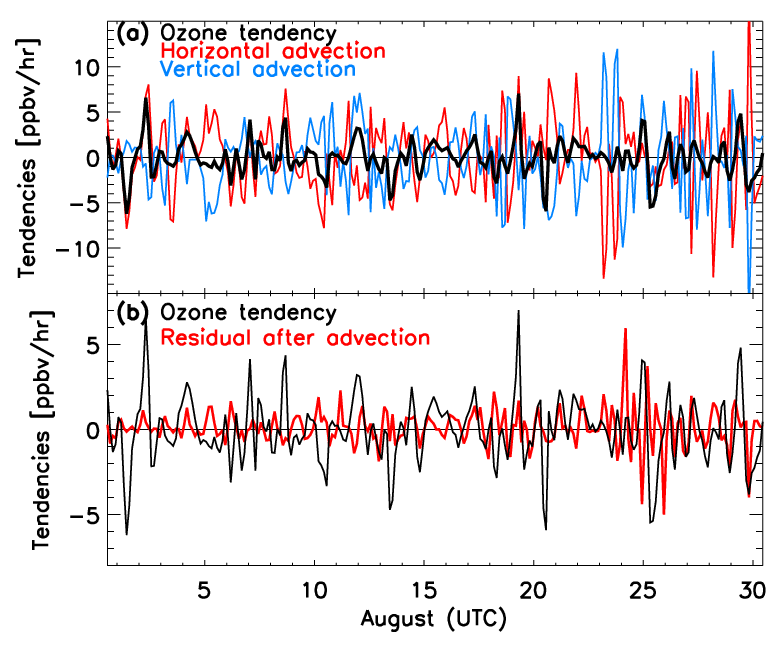
\includegraphics[width=0.48\textwidth]{tendency/residual}
		\caption[Ozone advective tendency]{{\small\textbf{Ozone advective tendency} --- Ozone tendencies and ({\bf a}) advective tendencies
		and ({\bf b}) residual tendencies after removing advective tendencies between 200--600\,\unit{hPa}. \vspace{-.2in}}}
		\end{singlespacing}
	\end{wrapfigure}

\figuremacroW{tendency/timeseries.png}{Time series for upper tropospheric tendency diagnostics}{\label{fig:2006/tendency_timeseries}
Time series at ({\bf a}) Trinidad Head, ({\bf b}) Houston, and ({\bf c}) Beltsville showing the min-mean-max ozone time series (black)
between 270--330\,\unit{hPa} overlaid with IONS-06 ozonesonde measurements represented as red vertical lines for the range and solid
$\diamondsuit$ for the mean value. Lightning \chem{NO_x} decaying tracer (cyan) and ozone chemical (red), convective (blue), and vertical
mixing (purple) tendency components are given according to the blue axis labels on the right in units of \unit{ppbv/3\,hr}. Boundary layer (BL, blue)
and stratospheric (ST, red) are also given in \unit{\%}.}{0.9}

The primary sources for local temporal variabilities are horizontal advection and vertical advection. Figure~\ref{fig:2006/tend_residual} shows
the advective tendencies for ozone compared to the total ozone tendency sampled near Houston between 200--600\,\unit{hPa}.
Both the horizontal and vertical components are often on the same magnitude as the total tendency. However, the combined
advective tendency is frequently much smaller because the two components are often anti-correlated with opposite signs. The residual
tendency, i.e. the total ozone tendency without the two advective components, can be accounted for by chemical, convective, and
vertical mixing tendencies. It is useful to note that the residual is not guaranteed to be smaller than the total tendency due to the ability for advective tendencies
to ``cancel'' out the effect of the remaining three components, as seen after August 23.

To characterize the residual tendency of the continental inflow, the anticyclone, and the continental outflow, three locations are selected to be
examined further: Trinidad Head, California (40.80$^\circ$N, 124.15$^\circ$W), Houston, Texas (29.72$^\circ$N, 95.30$^\circ$W),
and Beltsville, Maryland (39.04$^\circ$N,76.52$^\circ$W). Figure~\ref{fig:2006/tendency_timeseries} shows the time series of the
ozone VMRs at these locations as well as the associated chemical, convective, and mixing tendencies. Values shown are the mean values for
all data points between 270--330\,\unit{hPa}, with min/max also indicated for ozone VMR.
To account for the model bias, IONS-06 ozonesonde measurements, described in Section~\ref{ssec:2006/gen/ozone}, are also included.
Boundary layer (BL), stratospheric (ST) and lightning (\lnox) decaying tracers, described in Section~\ref{ssec:2006/discuss/tracer}
, are included to provide context of the sources for the dynamical and chemical variabilities.

Trinidad Head periodically receives stratospheric ozone from the northern latitudes, which is responsible for the sharp spatiotemporal gradients
of high ozone simulated for particular days (e.g. August 2 and August 7). The largest 3-hourly chemical tendency for Trinidad Head is
$0.37\,\unit{ppbv}$ per 3 hours. Similar to chemical tendency, convective and vertical mixing tendencies are also negligible, and thus advective tendencies dominate
the ozone variability in this region with a mean 3-hourly absolute advective tendency of $8.28\,\unit{ppbv}$ per 3 hours. On the other hand,
ozone has the highest chemical tendencies at Houston, with minimum/maximum values of
$-12.8/17.1\,\unit{ppbv}$ per 3 hours. The corresponding minimum/maximum values at Beltsville are $-2.94/3.90\,\unit{ppbv}$ per 3 hours. However, due to less frequent
negative (or loss) phases, the accumulated chemical tendency at Beltsville is higher than that at Houston, with a value of $110\,\unit{ppbv}$
compared to $69\,\unit{ppbv}$ over August.

Both convective and mixing tendency components are small at all three locations, with accumulated values (over August) of $-13.4\,\unit{ppbv}$ convective
and 3.6\,\unit{ppbv} mixing at Houston, -5.1\,\unit{ppbv} convective and 3.5\,\unit{ppbv} mixing at Beltsville, and -2.0\,\unit{ppbv} convective and
8.1\,\unit{ppbv} mixing at Trinidad Head over the entire August. The relatively larger value of vertical mixing tendency at Trinidad Head can be
attributed to the jet stream, which provides large vertical gradient in ozone VMR. For convection, detrainment of ozone-poor BL
air causes ozone to be diluted and thus the convective component is predominately negative.

	\begin{figure}[t!]
		\centering
		 \label{fig:2006/tendency_vertical} 
		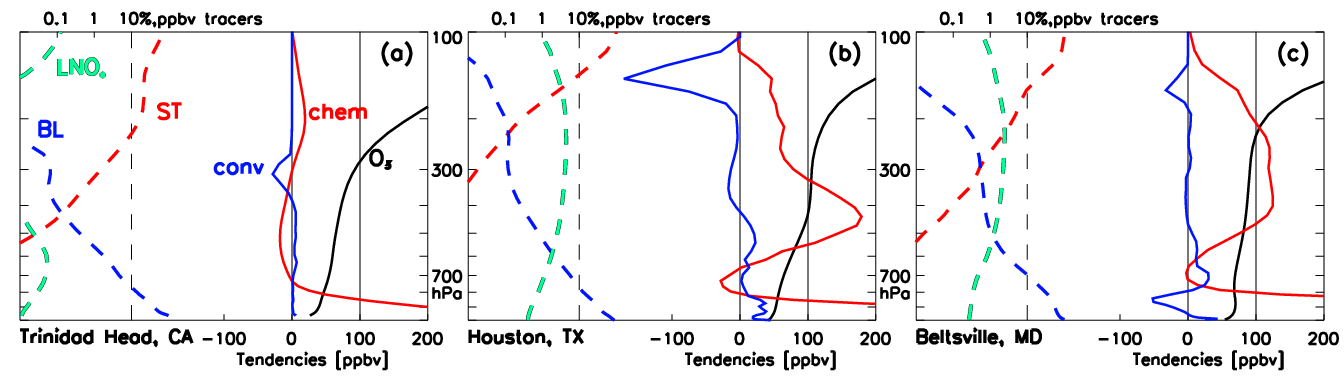
\includegraphics[width=1.0\textwidth]{tendency/vertical.png}
		\caption[Vertical profiles of decaying tracers and tendency diagnostics]{\textbf{Vertical profiles of decaying tracers
		and tendency diagnostics} --- August vertical profiles at ({\bf a}) Trinidata Head, ({\bf b}) Houston,
		and ({\bf c}) Beltsville. Dashed lines are the mean 1-d decaying tracers for BL (blue, \unit{\%}), ST (red, \unit{\%}), and {\lnox} (cyan,
		\unit{ppbv}) according to the values of the top axis. Solid lines are the accumulated chemical tendency diagnostic (red), convective
		tendency diagnostic (blue), and mean ozone profiles in \unit{ppbv} according to the values of the bottom axis. Closest $11\times11$
		grid points to the IONS-06 site are selected to compute these profiles.}\vspace{-.3in}
	\end{figure}

Figure~\ref{fig:2006/tendency_vertical} shows the vertical profile of the mean decaying tracers and accumulated tendencies within 5 grids
($11\times11$) surrounding the IONS-06 sites from August 1 00\,\unit{UTC} to August 31 00\,\unit{UTC}. The inflow region (Trinidad Head)
lacks both BL air and {\lnox} in the upper troposphere. Despite comparable ozone level to the other two locations, the accumulated tendency in the upper
troposphere remains low with a maximum of $19.4\pm2.5\,\unit{ppbv}$. Because of the lack of in-situ chemical production, the ozone level remains
low between stratospheric intrusion episodes, allowing the air to remain relatively ``clean'' until reaching Minnesota (Fig.~\ref{fig:2006/o3_300}).
This influx of low-ozone, chemically-``slow'' air mass between each stratospheric event is therefore responsible in generating the oval-shaped
ozone enhancement that trace the mean circulation in the seasonal average.

At Houston, at the center of the mean-state anticyclone, both the ozone chemical and convective tendencies are substantially higher than Trinidad Head.
At 200\,\unit{hPa}, where Trinidad Head records the peak net upper tropospheric ozone production, Houston records $55.8\pm18.6\,\unit{ppbv}$, about
2.9 times higher. However, this number, as discussed earlier, has been suppressed due to large negative phases of the diurnal cycle, which are caused by
large amount of BL air and {\lnox} as indicated by the tracers. Ozone-poor air is transported into the upper troposphere through
convection, detraining primarily at 145\,\unit{hPa} with a net change of $-170\,\unit{ppbv}$ \chem{O_3} during August, in part
caused by a nearby outlier with $-1170\,\unit{ppbv}$\footnote{Localized high convective tendency is an indication for stationary features such as sea
breeze or orographically triggered convections.} during August. However, the chemical maximum above the BL occurs in the mid-troposphere at
$437\pm2\,\unit{hPa}$ with a net production of $178\pm51\,\unit{ppbv}$ of \chem{O_3}. The position of this peak can be explained by the coincidence of the maximum
level for the prescribed {\lnox} emission based on \citet{Ott:2010lo} and the availability of BL air. As a consequence of production at this level, the mean
ozone VMR exceeds 100\,\unit{ppbv} at 437\,\unit{hPa}. In contrast, without {\lnox}, ozone loss via chemistry is expected at this level as
demonstrated at Trinidad Head.

In the outflow region, as represented by Beltsville, there is a higher net in-situ production of ozone in the upper troposphere despite having lower
ozone mixing ratios in the mid-to-upper troposphere compared to Houston. This can be attributed to having less frequent negative phases that destroy ozone at night. Despite the smaller net
convective tendency, the BL tracer is higher than or comparable to the Houston column, indicating that ozone precursors are advected from elsewhere. An
in-depth analysis of the ozone budget and variability at this location and New England can be found in \citet{Thompson:2007gd,Thompson:2007ov}, which 
utilizes IONS-04, the predecessor of IONS-06. They found that tropospheric ozone in northeastern North America was composed of 10--15\% BL sources,
10--15\% regional sources including lightning, 20--25\% stratospheric ozone, and $\sim50\%$ recently advected or aged air from elsewhere.

%\subsubsection{Chemical pathways}
%
%The approach above cannot be used to attribute the simulated chemical tendency to the appropriate chemical pathway. Considering the nonlinear
%dependency of ozone
%production/loss on the atmospheric composition, higher-ordered relation needs to be examined. For urban pollution, the Empirical Kinetic Modeling
%Approach (EKMA) has been used to estimate the ozone isopleths in relation to VOC and \chem{NO_x} ratio \citep{Dimitriades:1977fk}. However, this model
%suffers several deficiencies, including the lack of dependency on temperature, solar radiance, and transport, all of which can substantially impact the
%rates of the presumed ozone steady state. By incorporating simple trajectories and taking into account location and time information, EPA's
%OZIPR\footnote{Research-oriented Ozone Isopleth Plotting Package (OZIPP)}model can compute ``city-specific'' EKMA, which is used by
%planners to achieve National Ambient Air Quality Standards (NAAQS) compliance and developers to construct research models.
%
%\figuremacroN{tendency/chem_EKMA}{Ozone chemical tendency in relation to \chem{NO_x}}{\label{fig:2006/nox_EKMA}
%Ozone chemical tendency in relation to \chem{NO} and \chem{NO_2} chemical tendencies between 15 and 21\,\unit{UTC} in August near Houston, TX
%at 200--600\,\unit{hPa} \vspace{-.2in}}
%
%Similar to EKMA, but instead of relating ozone VMR to species VMRs, here we relate ozone to relevant species within the anticyclone
%using their chemical tendencies. Figure~\ref{fig:2006/nox_EKMA} shows the net ozone production between each 3-hourly output given
%\chem{NO} and \chem{NO_x} chemical tendency during daytime (15--21\,\unit{UTC}) and within 5 model grids from the IONS-06 Houston
%launch site at heights with August mean pressure 200--600\,\unit{hPa}. The \chem{NO}+\chem{NO_2} chemical tendency is generally
%negative, thus indicating that non-\chem{NO_x} nitrogen species are being produced, e.g. \chem{NO_3}, \chem{HNO_4}, \chem{HONO},
%which can explain the strong nocturnal loss phase in ozone. However, this does not guarantee a negative overall \chem{NO_x} tendency
%due to \chem{NO} emission from lightning. Finally, ozone production is generally small when the \chem{NO_x} tendency is small (close to the
%steady state line), and ozone production occurs when  $\Delta_{chem}\chem{NO}$ is negative while $\Delta_{chem}\chem{NO_2}$ is small.
%
%Since the chemical tendency is fundamentally tied to the chemical mechanism, i.e. the available chemistry set, it is possible to generalize this distribution to other
%locations at the same local time\footnote{This requirement guarantees similar photolysis rates ignoring the presence of shadows from deep convective clouds.}
%using only a subset of chemical tendency diagnostics. Let $\mathbf{x}$ be a feature vector of length 8, where $x_0=1$ and $x_1\ldots x_5$ be the chemical
%tendencies for \chem{CO}, \chem{NO_x}, and \chem{HO_x} in \unit{ppbv/hr}. Chemical tendency for ozone which is designated as $y$. Using a least-square
%regression with $L^2$-regularization parameter $\lambda=1$, we fit the following function to the Houston daytime data:
%\begin{equation}\label{eqn:chem_ekma}
%	y = \mathbf{x}\mathbf{A}\mathbf{x}^T
%\end{equation}
%where $\mathbf{A}=\{a_{ij}\}_{i,j}$ is a $6\times6$ upper triangular matrix, $\mathbf{x}=(x_0,x_1,\ldots x_5)^T$. Table~\ref{table:2006/ekma_regress}
%shows the coefficients of $\mathbf{A}$ from a 100 bootstrap iterations trained on 40.8k (50\%) and tested on 40.8k (50\%) of the data points. The
%RMS errors for the regressions from the bootstraps are $0.2954\pm0.0008\,\unit{ppbv/hr}$. Applying the same fitted model to Beltsville gives RMS
%errors of $0.2651\pm0.0003$\,\unit{ppbv/hr}.
%
%	\begin{table}[htp!]
%	\caption[Quadratic regression on chemical tendencies]{Mean and standard deviations of the coefficient matrix $\mathbf{A}$ in
%	Equation~\ref{eqn:chem_ekma}. Insignificant terms where $M_{ij}=\max|\overline{a_{ij}}x_ix_j|<10^{-3}\,\unit{ppbv/hr}$ at Houston
%	are shown as $\sim0$, otherwise $\log M_{ij}$ are included in parentheses.}
%	\begin{center}
%	\begin{tabular}{|c|c|c|c|c|c|c|}\hline
%					& 1	& \chem{CO}			& \chem{NO}			&\chem{NO_2}		& \chem{HO}		&\chem{HO_2}			\\ \hline
%		1			& 0	& $-0.676\pm0.008$		& $-4.45\pm0.019$		&$-5.83\pm0.030$	& $0.484\pm0.031$	& $-9.33\pm0.147$		\\
%					&	& $(0.273)$			& $(0.689)$			& $(0.666)$		& $(-2.86)	$		& $(-0.543)$			\\ \hline
%		\chem{CO}	& -	& $-23.2\pm0.265$		& $0.549\pm0.014$		&$-0.206\pm0.048$	& $-1.10\pm0.086$	& $\sim0$				\\
%					& 	& $(-0.274)$			& $(0.625)$			& $(-0.398)$		& $(-0.080)$		& $(-3.02)$			\\ \hline
%		\chem{NO}	& -	& -					& $1.17\pm0.13$		&$2.87\pm0.22$	& $-2.40\pm0.06$	& $-2.57\pm0.16$		\\
%					&	&					& $(-1.32)$			& $(-1.01)$		& $(0.460)$		& $(0.351)$			\\ \hline
%		\chem{NO_2} 	& -	& -					& -					&$\sim0$			& $0.668\pm0.075$	& $9.50\pm0.13$		\\
%					&	&					&					&				& $(-1.94)$		& $-0.827$			\\ \hline
%		\chem{HO}	& -	& -					& -					& -				& $-2.92\pm0.13$	&$\sim0$				\\
%					&	&					&					&				& $(0.267)$		&					\\ \hline
%		\chem{HO_2}	& -	& -					& -					& -				& -				& $-1.60\pm0.05$		\\
%					&	&					&					&				&				& $-1.60$				\\ \hline
%	\end{tabular} \label{table:2006/ekma_regress}
%	\end{center}
%	\end{table}
%
%The model represented by Table~\ref{table:2006/ekma_regress} should be applicable for chemical compositions within or near the domain encompassed by
%the data from Houston. Let $M_{ij}=\max_{ij}|\overline{a_{ij}}x_ix_j|$ be the maximum tendency contribution to the net ozone tendency. At Houston, the
%largest components are \chem{NO} and \chem{NO_2}, with $\log M_{ij}=0.689$ and 0.666 respectively. Due to the compositions, $M_{ij}$'s may have different
%upper bounds at different locations. Applying the same model to Beltsville, $\log M_{ij}=0.833$ and 1.041 respectively. The largest differences, however, are in
%the components $\langle\chem{HO},\chem{HO}\rangle$, $\langle\chem{NO},\chem{HO}\rangle$ and $\langle\chem{NO},\chem{HO_2}\rangle$, of which the $\log
%M_{ij}$'s evaluate to 0.267, 0.460, 0.351 at Houston but 1.016, 0.748, 0.869 at Beltsville, representing a combined $3.3\times$ maximum contribution to the
%variability of ozone production by the interactions between \chem{HO_x} and \chem{NO}. The reason for this difference is not due to changes in chemistry, but
%the differences in the domain spanned by $\mathbf{x}$, which effectively selects a subset of the mapped ozone tendency values.

\section{Sensitivity study}\label{sec:2006/sens}

There are numerous variables in the base case simulations that could have contributed to the model biases as evaluated in Section~\ref{sec:2006/general}. In
particular, the emission and distribution of lightning-generated \chem{NO_x} (\lnox) have been shown to be a significant component in determining the
atmospheric composition in the free troposphere as represented by CTMs \citep{Labrador:2005uq,Cooper:2009nx,Ott:2010lo}. Thus it is useful to perform
sensitivity simulations to determine the range of variabilities caused by the uncertainties and biases in the lightning parameterization.

Other than the lightning-generated \chem{NO} emission, anthropogenic and biogenic emissions are also crucial in determining the atmospheric composition. While having a lesser
degree of uncertainty and sensitivity compared to {\lnox}, urban developments and policy changes can have substantial impacts on the emission inventory
(Sect.~\ref{ssec:intro/ozone/nox}). As such, sensitivity studies on anthropogenic and biogenic emissions are valuable in determining the calibration
requirements for hypothetical scenarios that correspond to potential changes.

\subsection{Lightning emission}\label{ssec:2006/sens/lnox}

The comparison to NLDN flash counts shows that the current lightning parameterization is producing an order of magnitude higher overall flash rates
(Sect.~\ref{ssec:2006/gen/met}). Two simulations are performed to account for the effect of overpredicting lightning flash rate, as well as to evaluate
the sensitivity of the ozone enhancement to the {\lnox}. These two simulations are identical to the base case simulation in Section~\ref{sec:2006/general}
except with lightning tuning parameter set to $0\times$ and $0.1\times$ to represent a control (no lightning) scenario and tuned-lightning scenario. The
resulting spatial distributions of several species at 300\,\unit{hPa} are shown in Figure~\ref{fig:2006/ltngsens_map}.

\figuremacroW{sens/ltngsens.png}{Upper tropospheric sensitivity to lightning}{\label{fig:2006/ltngsens_map}
Model simulated mean {\bf(a)} \chem{O_3}, {\bf(b)} \chem{CO}, {\bf(c)} \chem{NO_x}, and {\bf(d)} \chem{HO_x} for $0\times$ (left column), $0.1\times$ (center column), and $1\times$ (right column)
lightning flash rate at 300\,\unit{hPa} for August. Note that \chem{NO_x} is contoured in the $\log$-scale.}{0.9}

% NOx
\chem{NO_x} is substantially increased above background values ($31.6\pm4.5\,\unit{pptv}$) to $135\pm35\,\unit{pptv}$ with $0.1\times$ lightning and
$1680\pm540\,\unit{pptv}$ with $1\times$ lightning. Modeling the contribution of total \chem{NO_x} mixing ratio by lightning-generated \chem{NO_x} as follow:
\begin{equation}\label{eqn:nox+lnox}
	\Delta[\chem{NO_x}] = [\chem{NO_x}]-[\chem{NO_x}]_0 = (1-p)[\chem{LNO_x}]
\end{equation}
where $p$ is the percentage loss of {\lnox} in the atmosphere and $[\chem{NO_x}]_0$ is the no-lightning \chem{NO_x} VMR. For small changes in the
atmospheric composition, $p$ should be constant and thus the addition of {\lnox} should linearly increase $[\chem{NO_x}]$. Falsely extrapolating this
to $1\times$ flash rate, the expected $[\chem{NO_x}]$ would have been $1070\,\unit{pptv}$. However, because of the decrease in \chem{HO_x}, the
primary reagent converting \chem{NO_x} into reservoir species, in response to {\lnox}, $\partial p/\partial [\chem{NO_x}] < 0$, and thus giving us the
simulated $1680\,\unit{pptv}$, higher than the linearly extrapolated value.

% HO_x
Unlike \chem{NO_x}, \chem{HO_x} is substantially decreased with increasing {\lnox} emission. The initial August mean VMR at 300\,\unit{hPa} without
lightning is $6.94\pm0.38\,\unit{pptv}$ within the anticyclone. This is above the $\sim$4--5\,\unit{pptv} in the Pacific Northwest and inflow regions. It is slightly decreased
to $6.27\pm0.37\,\unit{pptv}$ with $0.1\times$ lightning, or a 10\% decrease from the $0\times$ scenario. At $1\times$ {\lnox} emission, \chem{HO_x}
is further decreased to $1.80\pm0.59\,\unit{pptv}$, far below the value to the northwest, representing a 71\% drop relative to the $0.1\times$ scenario,
which is larger than that would have been obtained if one ($\sim61\%$) were to extrapolate the initial 10\% decrease with an exponential model.
The decreasing \chem{HO_x} with increasing \chem{NO_x} is the results of its interactions with \chem{O_3}, \chem{NO_x}, and \chem{CO} after production
from the \chem{O(^1D)+H_2O}, which is presumably proportionally increasing with the increased level of \chem{O_3}. However, because the VMRs
of all species have been perturbed as the result of {\lnox} emission, it is challenging to describe the new mean \chem{HO_x} with {\lnox} relative to
the control state with $0\times$ lightning.

% CO
Even though \chem{CO+OH\rightarrow CO_2+HO_2} is the only chemical loss pathway for \chem{CO} specified in RADM2 and that \chem{HO_x} is
substantially decreased by a factor of 3.8 from $0\times$ to $1\times$ lightning, \chem{CO} decreases with increasing lightning. Without lightning, the
August mean anticyclone VMR for \chem{CO} is $92.3\pm2.8\,\unit{ppbv}$. This is reduced to $89.8\pm.2.4\,\unit{ppbv}$ with $0.1\times$ lightning
and $85.5\pm2.4\,\unit{ppbv}$ with $1\times$ lightning. The anti-correlation of \chem{CO} with {\lnox} can be described by the dominating effect of
reduced in-situ production of \chem{CO} from \chem{(HCHO,GLY,MGLY)+OH} over increased production from \chem{(OL2,OLT,OLI,ISO)+O_3}.
\footnote{\chem{OL2}=ethene; \chem{OLT}=terminal alkenes; \chem{OLI}=internal alkenes.}

% O3
Finally, \chem{O_3} is increased with increasing {\lnox}, consistent with prior studies on this subject. Mean ozone VMR
is increased from $74.5\pm5.3\,\unit{ppbv}$ to $86.4\pm6.7\,\unit{ppbv}$ ($+16\%$) when adding $0.1\times$ {\lnox}. At $1\times$ lightning, it
is further increased to $101.1\pm6.8\,\unit{ppbv}$, a $26.6\,\unit{ppbv}$ or $36\%$ increase relative to $0\times$ lightning. The reduced sensitivity
to {\lnox} at higher flash rate parameter is consistent with that of \chem{CO}.

There is also a difference in the spin-up time for species in responding to {\lnox} emission due to their respective lifetime in
the atmosphere While the differences in \chem{NO_x} between simulations become apparent within the first day, \chem{HO_x} requires 
two days, which is delayed by a separate spin-up from exchanging between \chem{HO_x} and reservoir species. On the other hand,
\chem{O_3} and \chem{CO} begin to diverge after the fifth day of the simulation when the $Z_{300}$ exceeded 9730\,\unit{m} for the first
time.  However, even after sufficient ``spin-up,'' the differences between simulations can be reduced again when air masses with minimal lightning
influence are transported into the region.

%o3:       74.4501      5.28160
%co:       94.2718      2.77095
%NOx:       31.5665      4.48547
%HOx:       6.93762     0.378603

%o3:       86.4036      6.68674			(+11.9) +16%
%co:       89.8467      2.38789			(-4.5)
%NOx:       135.365      34.9208			(+103.4)
%HOx:       6.27117     0.368946		(-0.666)

%o3:       101.067      6.79265			(+14.6)
%co:       85.4519      2.37563			(-4.3)
%NOx:       1678.35      535.866			(+1543)
%HOx:       1.79844     0.585140		(-4.473)

	\begin{figure}[t!]
		\centering
		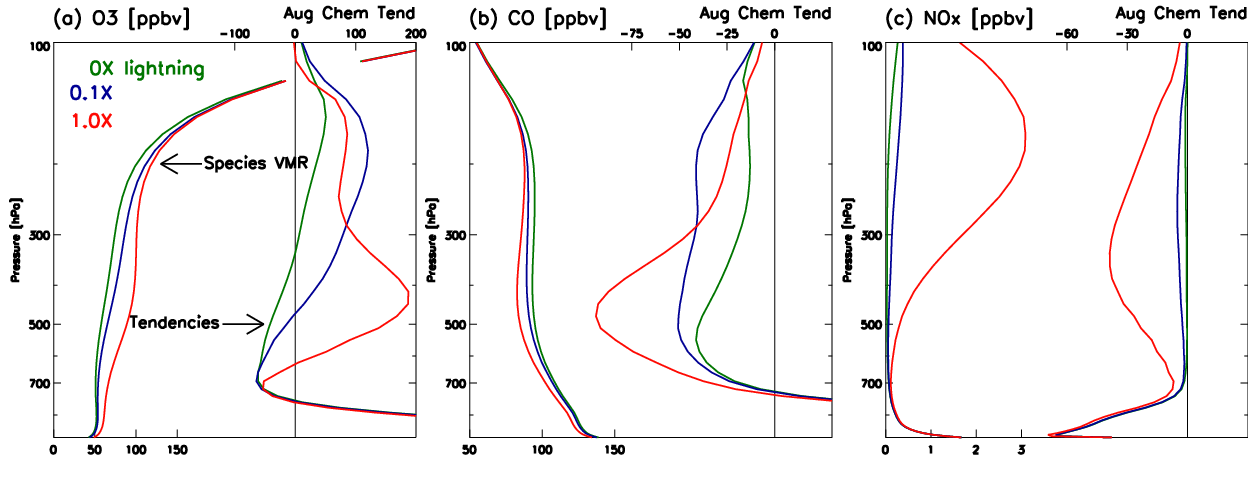
\includegraphics[width=1.0\textwidth]{sens/ltngsens_vert.png}
		\caption[Vertical sensitivity profiles of \chem{O_3}, \chem{CO}, \& \chem{NO_x} to lightning]{\textbf{Vertical
		profiles of \chem{O_3}, \chem{CO}, \& \chem{NO_x}} --- August mean mixing ratios and
		accumulated chemical tendencies for {\bf(a)} \chem{O_3}, {\bf(b)} \chem{CO}, {\bf(c)} \chem{NO_x} within the anticyclone
		region for lightning emission factors $0\times$ (green), $0.1\times$ (blue), and $1\times$ (red). Means are
		computed on model levels, and then gridded by the mean pressure.
		\label{fig:2006/ltngsens_vertical} }\vspace{-.3in}
	\end{figure}

Vertical structures are also affected. Figure~\ref{fig:2006/ltngsens_vertical} shows the vertical sensitivity profiles of ozone,
\chem{CO}, and \chem{NO_x}. With the exception of \chem{O_3} and \chem{NO_x} in the $1\times$ lightning setting, the
shapes of species VMR vertical profiles are consistent across simulations. Peak of ozone enhancement from
$0\times$ to $1\times$ lightning occurs between 300--500\,\unit{hPa}, with a maximum mean \chem{O_3} enhancement
of 33.3\,\unit{ppbv} ($\Delta_{chem}\chem{O_3}=187\,\unit{ppbv}$) above the control state of 61.7\,\unit{ppbv}
($\Delta_{chem}\chem{O_3}=-29\,\unit{ppbv}$) at 445\,\unit{hPa}. Despite emission peak in the mid-troposphere,
\chem{NO_x} is enhanced most prominently at 169\,\unit{hPa} from 84\,\unit{pptv} to 3.09\,\unit{ppbv}. A more detailed
discussion of this peak and its spin-up has been discussed in Section~\ref{ssec:2006/gen/nox}.

On the other hand, \chem{O_3} and \chem{CO} chemical tendencies show highly nonlinear response to lightning emission
despite monotonic increases in the magnitude of \chem{NO_x} chemical losses. Due to the increase in ozone production
from {\lnox} in the mid-troposphere, altitude at which positive net \chem{O_3} attained within the anticyclone is gradually
decreased from the initial $\sim340\,\unit{hPa} $ in the control simulation to $\sim470\,\unit{hPa}$ with $0.1\times$ {\lnox},
and finally $\sim630\,\unit{hPa}$ in the $1\times$ scenario. This is the pressure level at which the ozone enhancement
is expected to reach, but not necessarily indicating the maximum enhancement because of transport.

In the upper troposphere, where \chem{NO_x} shows superlinear increases due to {\lnox} between $0.1\times$
and $1\times$ lightning, suggesting feedback. Consequently, the presence of high \chem{NO_x} induces reversal in the chemical production
of \chem{O_3}. \chem{NO_x} titration has been suggested to be possible during intense thunderstorms \citep[e.g.][]{Cummings:2013vn}.
However, persistent occurrence indicated in Figure~\ref{fig:2006/ltngsens_vertical} is in part due to overestimation of
\chem{NO_x} as a result of the $10\times$ over-prediction in lightning flash rate. On the other hand, with the increased
\chem{NO_x} VMR, \chem{HO_x} radicals are consumed for the reaction \chem{OH+NO_2\rightarrow HNO_3},
thus negatively affecting the efficiency of \chem{NO}-to-\chem{NO_2} conversion.

Figure~\ref{fig:2006/ltngsens_distr} isolates daytime production from nighttime loss from the overall accumulated tendency shown
in Figure~\ref{fig:2006/ltngsens_vertical} between 150--300\,\unit{hPa} within the anticyclone. Daytime tendencies are computed
from 15--21\,\unit{UTC} and nighttime tendencies are computed from 3--9\,\unit{UTC}. The daytime/nighttime differences for species
VMR is minimal, and thus only daytime VMR distributions are shown. In conjunction with the mean values, the min-max ranges as well as the
5--95 percentiles are shown. Due to the interconversion between \chem{O_3} and \chem{NO_2}, we examine odd oxygen
\chem{O_x\equiv O_3+NO_2} instead of \chem{NO_2} in the following analysis.

\figuremacroN{sens/ltngsens_diurnal}{Daytime and nighttime chemical tendencies}{\label{fig:2006/ltngsens_distr}
Distributions (min-5pct-mean-95pct-max) of chemical tendencies mixing ratios for \chem{O_3}, \chem{O_x}, \chem{CO} and
mixing ratio for \chem{HNO_3} between 150-300\,\unit{hPa} during August within the anticyclone. Nighttime tendencies are
represented by dashed lines while daytime tendencies are represented by solid lines.}

While the differences between ozone VMRs between scenarios are monotonic and small ($<25\%$) between the $0\times$
and $1\times$ experiments, chemical tendencies between scenarios show staggering changes with the addition of {\lnox}. Without lightning,
mean daytime chemical tendency is simulated to be 0.088\,\unit{ppbv/hr} and the 95-percentile is 0.259\,\unit{ppbv/hr}. With the
addition of $0.1\times$ {\lnox}, the mean and 95-pct respectively increases to 0.353\,\unit{ppbv/hr} and 0.904\,\unit{ppbv/hr}. Due to
the transient nature of {\lnox} influence, and the relatively short lifetime of \chem{NO_x}, the distributions of the tendencies are
also less homogeneous. Increasing {\lnox} emission by 10-fold to the ``base'' case, daytime mean chemical tendency for \chem{O_3}
is slightly increased to 0.403\,\unit{ppbv/hr}, as opposed to the decrease in the all-day accumulated profiles. On the other hand, ozone
loss/reduced production are shown in the low-end of the distributions, where the 5-percentile is decreased from 0.042\,\unit{ppbv/hr}
to 0.033\,\unit{ppbv/hr} and the minimum (largest potential loss) is decreased from $-0.093$ to $-0.853\,\unit{ppbv/hr}$, thus 
supporting the conjecture that daytime \chem{NO_x}-titration is indeed occurring albeit not as severe as indicated in
Figure~\ref{fig:2006/ltngsens_vertical}. By inspecting the \chem{O_x} tendency, it is further shown that the additional ozone loss
is due to conversion to \chem{NO_2}. Nonetheless, loss to \chem{HNO_3} is significant, $[\chem{HNO_3}]$ is doubled from 3.3\,\unit{ppbv}
without lightning to 6.6\,\unit{ppbv}. This is further increased to 39.6\,\unit{ppbv} at $1\times$ lightning, i.e. a $12\times$ increase
for $10\times$ {\lnox} emission.

The remainder of the reversal in the response of the \chem{O_3} chemical tendency to {\lnox} after considering the
daytime production is evidently substantial. Due to the absence of photolysis, the nighttime maximum tendencies
are all near zero. Without production, we can define zero as the baseline and evaluate the sensitivities as
relative changes. In the $0\times$ scenario, the ozone loss is 0.90\,\unit{pptv/hr} with the 5 percentile at 2.93\,\unit{pptv/hr}.
The mean loss is increased to 5\,\unit{pptv/hr} ($5.6\times$) and the 5 percentile is increased to 25.8\,\unit{pptv/hr}
($8.8\times$) with $0.1\times$ {\lnox}. Increasing {\lnox} to $1\times$, the mean is now 48.2\,\unit{pptv/hr}, a $9.5\times$
increase from the low(tuned)-lightning scenario, i.e. slightly sublinear compared to the increase in emission. The
negative-end of the distribution, on the other hand, shows linear responses at both 5-percentile ($-0.0258\rightarrow-0.259\,\unit{ppbv/hr}$)
and minimum ($-0.179\rightarrow-1.78\,\unit{ppbv/hr}$) from $0.1\times$ to $1\times$ emissions. However, the response
is not linear for the tendency for \chem{O_x} because of the potential for production (positive tendency) of \chem{NO_2}
at nighttime, which is negligible with no lightning ($\max\Delta = 8\times10^{-2}\,\unit{pptv/hr}$), but increases to 79\,\unit{pptv/hr}
with $1\times$ lightning, which is comparable to the mean tendency ($-51\,\unit{pptv/hr}$). Despite production, response
to lightning emission has became superlinear relative to a baseline of zero, wherein the \chem{O_x} tendency for
the two lightning scenarios are $-4.3$ and $-51\,\unit{pptv/hr}$. This points to loss of odd oxygens via both \chem{O_3} and
\chem{NO_2} pathways at night.

	\begin{figure}[t!]
		\centering
		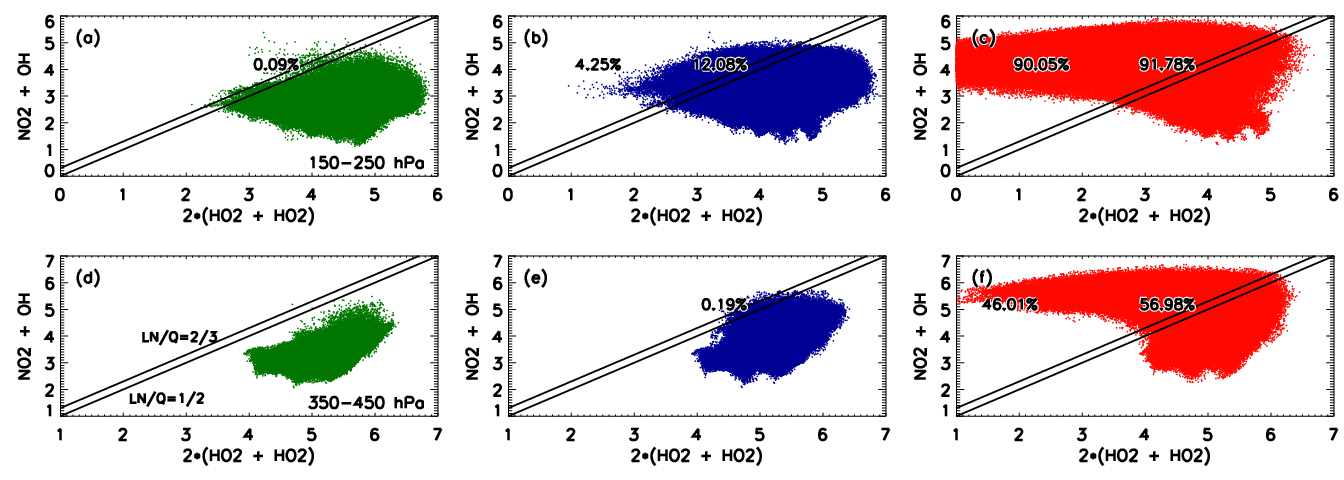
\includegraphics[width=1.0\textwidth]{sens/rxn}
		
		\caption[\chem{HO_x} radical termination]{\label{fig:2006/ltngsens_rxn}\textbf{\chem{HO_x} radical termination}
		--- Daytime reaction rates ($\log_{10}\,\unit{molecules\,cm^{-3}\,s^{-1}}$) for \chem{NO_2+OH} and ($2\times$)
		\chem{HO_2+HO_2} at 150--250\,\unit{hPa} ({\bf a--c}) and 350--450\,\unit{hPa} ({\bf d--f}) without lightning ({\bf a,d}),
		$0.1\times$ lightning ({\bf b,e}), and $1\times$ lightning ({\bf c,f}). The left percentage (if present) is the fraction
		of data points where $L_N/Q>2/3$. The right percentage (if present) is that of $L_N/Q>1/2$.}\vspace{-.3in}
	\end{figure}

Since \chem{CO} precursors are generally scarce in the upper troposphere, and that \chem{OH} VMR is low at night,
neither production nor loss occur at appreciable rates. The nighttime \chem{CO} chemical tendency ranges from
-6.3\,\unit{pptv/hr} ($0.1\times$) to 2.7\unit{pptv/hr} ($1\times$). On the contrary, daytime \chem{CO} chemical tendency
shows a substantial range relative to its mean values. The middle 90\% spans $-109$--$80\,\unit{pptv/hr}$ without lightning,
with a mean of $-46\,\unit{pptv/hr}$. This indicates that a sufficient \chem{CO} precursors are present in the upper
troposphere to counter the loss due to reaction with \chem{OH} radical. The addition of $0.1\times$ lightning \chem{NO_x}
moves this range to $-281$--$3\,\unit{pptv/hr}$, thus doubling the net loss on the low end and essentially erased any
production. This is likely caused by loss of VOCs due to oxidation at lower levels, thus leaving less for in-situ \chem{CO}
production in the upper troposphere after transport. At $1\times$ {\lnox}, however, the lower-end tendency trend is
reversed and the net loss at 5-percentile is now $-255\,\unit{pptv/hr}$. These data points correspond to high-{\lnox} air
masses, in which \chem{OH} radicals are competitively consumed by \chem{NO_2} in the production of \chem{HNO_3}.
At 95-percentile, the trend continues to decrease, and it is now a net 3-hourly loss of $-25\,\unit{pptv/hr}$.

The response of ozone production to the available \chem{NO} can be quantified as follow \citep{Kleinman:2001fk}:
\begin{equation}\label{eqn:k01NO}
	\frac{d\ln P(\chem{O_3})}{d\ln[\chem{NO}]} = \frac{(1-3/2\,L_N/Q)}{(1-1/2\,L_N/Q)}
\end{equation}
where $L_N/Q$ is the fraction of \chem{HO_x} radicals, principle intermediates for ozone production, removed by
\chem{NO_x} as opposed to radical-radical reactions. In the upper troposphere, $L_N$ and $L_R=Q-L_N$ can be
approximated by the reaction rate of \chem{NO_2+OH} and twice the rate of \chem{HO_2+HO_2}. For consistency,
offline computations are performed using the rate equations and parameters from RADM2
\citep[][and references therein]{Stockwell:1990ez}. Using August data points at 15, 18, and 21\,\unit{UTC} within
the anticyclone column between 150--250\,\unit{hPa} and 350--450\,\unit{hPa}, the reaction rates
$L_N=k\chem{[NO_2][OH]}$ and $L_R=2k'\chem{[HO_2][HO_2]}$ are plotted in Figure~~\ref{fig:2006/ltngsens_rxn}.
The percentage of data points where $L_N>L_R$, or $L_N/Q > 0.5$, and $L_N/Q>2/3$ are computed at both
levels for all 3 lightning sensitivity simulations. This threshold indicates transition from \chem{NO_x}-limited to
VOC-limited regime. Suppressing lightning, almost all data points lies within $L_N/Q<0.5$. With $0.1\times$
lightning, about 12\% in the upper level exceeded this threshold, but almost all \chem{HO_x} below 350\,\unit{hPa}
continues to be terminated by radical-radical reactions. At $1\times$ lightning, 91.78\% and 56.98\% of the data
points are within the VOC-limited regime for the two pressure levels. If considering only those where the expected response of $P(\chem{O_3})$
to $[\chem{NO}]$ is negative, the percentages decrease to 90.05\% and 46.01\%. These numbers satisfactorily
explain the reversal in response observed in the upper troposphere (majority $L_N/Q>2/3$), and seemingly high
at the bottom of the enhancement (majority $L_N/Q<2/3$).

\figuremacroN{sens/ltngsens_o3conv}{Ozone convective tendency}{\label{fig:2006/ltngsens_o3conv}
Vertical profiles of accumulated ozone convective tendency during August for the three lightning sensitivity simulations
within the anticyclone column.}

Finally, due to changes in the vertical profile, and thus vertical gradients, convective tendencies are also affected by
lightning emissions (Fig.~\ref{fig:2006/ltngsens_o3conv}). While it still holds true that convection dilutes upper
tropospheric ozone by detraining air from the lower levels, changes in ozone due to convection exhibit are very different
below the maximum detrainment level between emission scenarios. In particular, due to the deeper enhancement (high
ozone at lower altitude), net negative convective tendency is observed above 440\,\unit{hPa} with $1\times$ lightning.
Lightning emission also impacts surface air quality through mid-to-upper tropospheric ozone enhancement, as observed
by the increasingly positive tendencies below 600\,\unit{hPa}. The accumulated ozone enhancement in the lower
troposphere is increased by 40--60\,\unit{ppbv} from $0\times$ to $1\times$ lightning despite relatively minimal local
chemical production (Fig.~\ref{fig:2006/ltngsens_vertical}{\bf a}).

\subsection{Anthropogenic emission}\label{ssec:2006/sens/anthrop}

	\begin{figure}[t!]
		\centering
		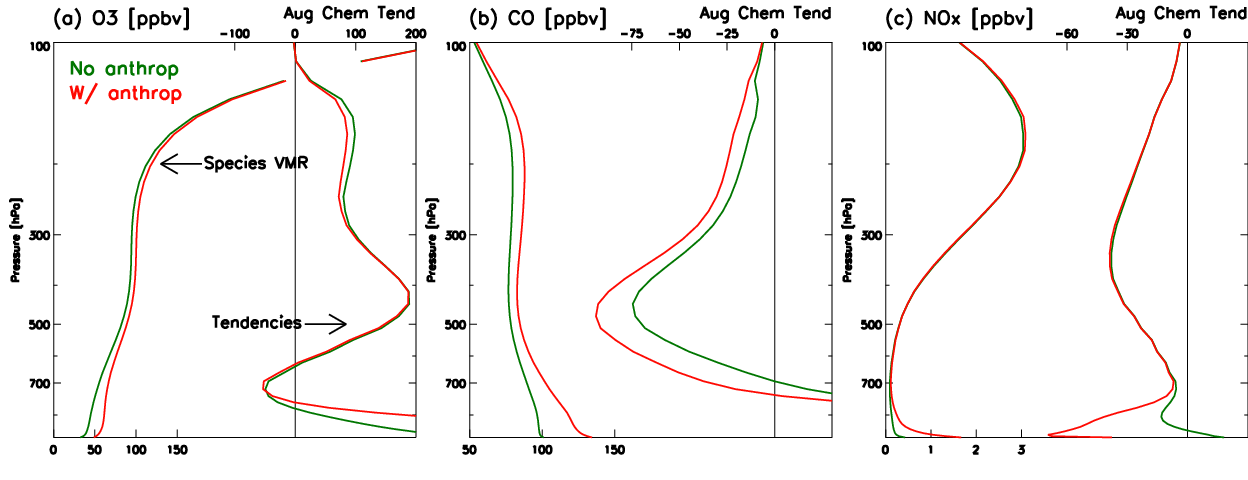
\includegraphics[width=1.0\textwidth]{sens/anthsens_vert}
		\caption[Vertical profiles for sensitivity to anthropogenic emission]{\textbf{Vertical profiles for sensitivity to
		anthropogenic emission} --- Same as Fig.~\ref{fig:2006/ltngsens_vertical}, but for anthropogenic emission.
		\label{fig:2006/anthsens_vert} }\vspace{-.3in}
	\end{figure}

To evaluate how anthropogenic emission affects the ozone enhancement, a simulation is performed without the prescribed
EPA emission. Lightning emission is kept at $1\times$, i.e. the untuned scenario. By cutting off anthropogenic emission, both
surface VOC and \chem{NO_x} sources are decreased. The differences ($[X]-[X]_0$) between the base case scenario and
the no-emission scenario are shown in Figure~\ref{fig:2006/anthsens}, where $[X]_0$ is the VMRs without emission, thus
a positive value represents an increase due to anthropogenic emission.

\figuremacroW{sens/anthsens}{Spatial distribution of sensitivity to anthropogenic emissions}{\label{fig:2006/anthsens}
Base case VMRs due to anthropogenic emission during August at 150, 300, and 450\,\unit{hPa} for ({\bf a--c}) \chem{O_3},
({\bf d--f}) \chem{CO}, and ({\bf g--i}) \chem{NO_x}. The differences are defined as VMRs without emission subtracted from
VMRs with emission. Geopotential height contour $Z_{300}=9730\,\unit{m}$ is shown at 300\,\unit{hPa}.}{0.9}

Within the anticyclone column at 300\,\unit{hPa} (Fig.~\ref{fig:2006/anthsens}{\bf b}), ozone due to anthropogenic emission
is $5.9\pm1.0\,\unit{ppbv}$ with a maximum of 7.8\,\unit{ppbv} with respect to a VMR $\sim100\,\unit{ppbv}$. Similarly,
sensitivity of \chem{CO} at 300\,\unit{hPa} to anthropogenic emission is $7.2\pm1.6\,\unit{ppbv}$ with a maximum of
11.5\,\unit{ppbv} (Fig.~\ref{fig:2006/anthsens}{\bf e}). The upper tropospheric \chem{O_3} and \chem{CO} responses
positively to anthropogenic emission, while \chem{NO_x} decreases with the addition of emission up to 300\,\unit{hPa}
but reverses at 150\,\unit{hPa}. Response of \chem{NO_x} at 150\,\unit{ppbv} is $54\pm34\,\unit{pptv}$. This is reversed
to $-19\pm9\,\unit{pptv}$ at 300\,\unit{hPa} but decreases in magnitude to $-1.3\pm6.7\,\unit{pptv}$, which is negligible
compared to the 1--3\,\unit{ppbv} VMR at these levels (for the $1\times$ lightning scenario).

At 150\,\unit{hPa}, all three species shown in Figure~\ref{fig:2006/anthsens} show maximum responses over Huntsville,
Alabama. This changes at 300\,\unit{hPa}, where two distinct maxima are shown for \chem{O_3} and \chem{CO},
corresponding to the maxima of \chem{CO} at northeast corner of Texas and along Blue Ridge Mountain as shown in
Figure~\ref{fig:2006/co_300}. On the other hand, \chem{NO_x} responses neutrally ($-2.3\pm8.0\,\unit{pptv}$) at
these locations relative to the surrounding area where negative responses are prevalent (Fig.~\ref{fig:2006/anthsens}{\bf h}).

Significant responses of chemical tendency to anthropogenic emission stops at $\sim700\,\unit{hPa}$ in the anticyclone
column mean (Fig.~\ref{fig:2006/anthsens_vert}). This sensitivity is then propagated into the upper troposphere through
convective transport, but the changes in BL air composition also allows moderate changes in the upper tropospheric
ozone production. As shown in Figure~\ref{fig:2006/anthsens_vert}{\bf c}, both \chem{NO_x} and \chem{NO_x} chemistry
are negligibly sensitive to anthropogenic emission with the prescribed level of {\lnox}, thus the changes in ozone chemical
tendency in Figure~\ref{fig:2006/anthsens_vert}{\bf a} is controlled by changes in \chem{CO} (or VOC) and its chemistry
(Fig.~\ref{fig:2006/anthsens_vert}{\bf b}).

\subsection{Biogenic emission}\label{ssec:2006/sens/bio}

Biogenic emission contributes significantly to tropospheric ozone production (see Sect.~\ref{ssec:intro/ozone/voc}).
Similar to anthropogenic emission, biogenic emission primary modifies the chemistry throughout the entire tropospheric
column through convective transport and chemistry.

	\begin{figure}[t!]
		\centering
		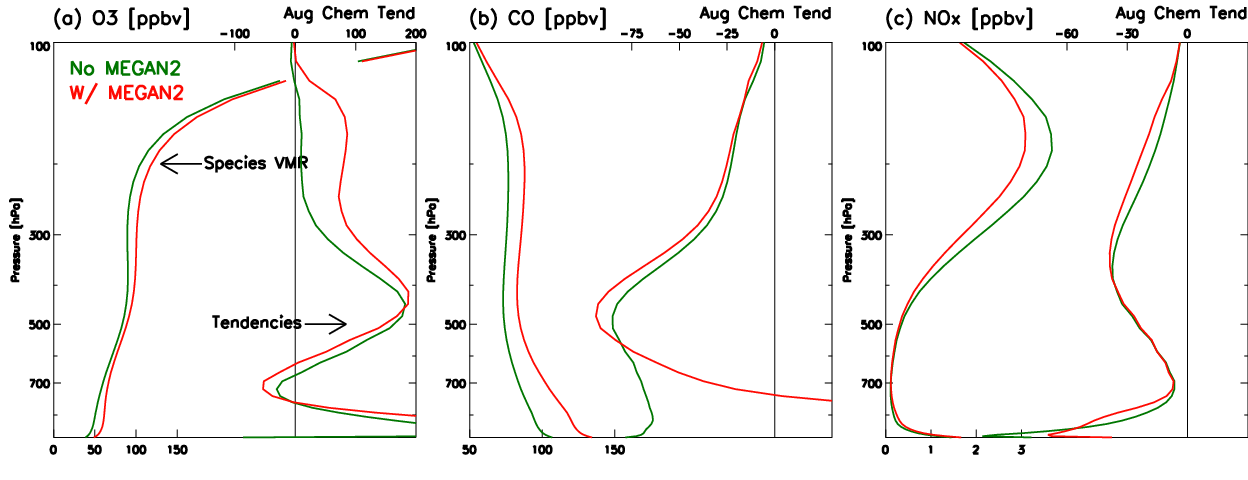
\includegraphics[width=1.0\textwidth]{sens/biosens_vert}
		\caption[Vertical profiles for sensitivity to anthropogenic emission]{\textbf{Vertical profiles for sensitivity to
		anthropogenic emission} --- Same as Fig.~\ref{fig:2006/ltngsens_vertical}, but for biogenic emission.
		\label{fig:2006/biosens_vert} }\vspace{-.3in}
	\end{figure}

To quantify the impact of biogenic emission on the upper tropospheric ozone and related chemistry within the anticyclone,
we subtract species VMR and chemical tendencies without biogenic emission from that with biogenic emission at
200\,\unit{hPa}, where ozone chemistry shows significant sensitivity to the absence of biogenic emission. At this level,
biogenic emissions enhances ozone by $13.4\pm3.2\,\unit{ppbv}$ as a result of $+69.6\pm37.5\,\unit{ppbv}$ accumulated
ozone chemical tendency over August. \chem{CO} has a similar change in VMR ($+11.2\pm2.6\,\unit{ppbv}$) from the
addition of biogenic emissions, but the enhancement is not in situ ($\Delta_{chem}=-2.3\pm4.6\,\unit{ppbv}$). On the other
hand, \chem{NO_x} experiences a decrease of $0.60\pm0.17\,\unit{ppbv}$ due to an increased accumulated loss of
$6.2\pm4.0\,\unit{ppbv}$.

Despite sharing the same originating level (BL) and transport pathways with anthropogenic emission sources, differences
in the emitted species composition and density are sufficient in producing different vertical profiles in the response. In
particular, ozone chemical tendency in the upper troposphere shows significant reduction when biogenic emission is
turned off. As opposed to being driven by VOCs as it is for anthropogenic emission, this change is due to the increased
\chem{NO_x} in the absence of biogenic emission (Fig.~\ref{fig:2006/biosens_vert}). In other words, the emission of
biogenic species such as isoprene and formaldehyde causes ozone to increase in the upper troposphere by decreasing
\chem{NO_x} within the \chem{NO_x}-titration regime (see Sect.~\ref{ssec:2006/sens/lnox}).


\newpage\section{Conclusions}\label{sec:2006/conslusion}

WRF-Chem simulations are performed with the goals of understanding the structure and chemical pathways of
the 2006 upper tropospheric ozone enhancement during the North American Monsoon. Using an untuned ($1\times$)
lightning based on a modified PR92 lightning flash rate parameterization, the predicted flash rate is about an order
of magnitude compared to the scaled NLDN history. This overestimation is shown to cause overly strong ozone
enhancement compared to TES and IONS-06 observation. On the other hand, \chem{CO} is shown to be either
biased high (against TES) or biased low (against MOPITT). However, it is shared in both validation exercises that
the simulated \chem{CO} distribution is more homogeneous than observed by either instruments.

Under the base case condition, the simulated \chem{NO_x} VMR is seen rapidly increasing within the first 5
days of the simulation by almost a factor of 10. As a consequence of the overprediction in {\lnox}, validation
against SCIAMACHY \chem{NO_2} retrieval shows that the model is simulating too much high \chem{NO_x}
events while properly predicting the mode of the distribution.

Tracer-tracer correlation using \chem{O_3} and \chem{CO} shows that the conditions within and outside of the
anticyclone are similar but differs in specific features. Using passive tracers, it is shown that the anticyclone region
distinguish itself by lateral boundary tracers and lightning tracers, and that boundary layer and stratospheric tracers
are dominated by orographic features instead of upper air circulation as suggested by previous studies. The
lack of externality, i.e. lack of influence of air mixing in from ``clean'' regions, and presence of both surface and lightning
emissions are thus concluded to be the key ingredients for the observed enhancement.

Other than enhanced ozone production, chemical and convective tendency within the anticyclone region also
show different structures compared to the continental inflow (Trinidad Head, CA) and outflow (Beltsville, MD)
regions. In particular, while mid-tropospheric net chemical loss (or minimal production) is observed outside
the anticyclone, maximum ozone production is simulated for this level, which subsequently lowers the level
at which in-situ ozone production is dominating transport and thus enhancing ozone VMR.

To quantify the impact of the uncertainties and biases of {\lnox} emission on the observed atmospheric composition
within the anticyclone, sensitivity simulations are performed by disabling emission ($0\times$) and tuning emission
($0.1\times$). Using the three simulations, it is concluded that the reduction of \chem{HO_x} radicals as a result of
increasing \chem{NO_x} causes the response of \chem{NO_x} to be superlinear to {\lnox}. By evaluating the
radical-termination pathways, it is also concluded that \chem{NO_x}-titration is indeed occurring at the level of
maximum \chem{NO_x} enhancement and thus reducing the potential ozone enhancement as a result of increasing
{\lnox}. Moreover, as a consequence of the modified vertical distribution responding to the changing {\lnox} emission,
convective tendencies are also modified.

Finally, control simulations for anthropogenic and biogenic emissions are performed to evaluate their contributions
to the ozone enhancement relative to the base case ($1\times$) scenario. While anthropogenic emission leads to
VOC-controlled changes, biogenic emission leads to major changes in upper tropospheric \chem{NO_x}. Since the
upper tropospheric chemistry is experiencing \chem{NO_x}-titration, the reduction of \chem{NO_x} (as a result of
biogenic emission) leads to a 70\,\unit{ppbv} increase in the August accumulated tendency at the detrainment level.